\documentclass{standalone}

\usepackage{tikz}

\begin{document}

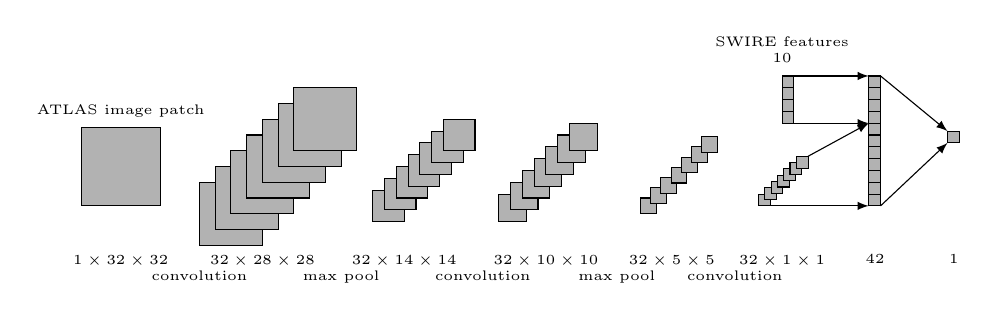
\begin{tikzpicture}
    % Inputs
    \filldraw[fill=black!30!white,
              draw=black] (0,0.5) rectangle (1,1.5);
    \draw (0.5, 0.0) node[anchor=north] {\tiny $1 \times 32 \times 32$};
    \draw (0.5, 1.5) node[anchor=south] {\tiny ATLAS image patch};
    % conv1
    \foreach \x in {0,...,6}
        \filldraw[fill=black!30!white,
                  draw=black] (1.5+0.2*\x,0.2*\x) rectangle (1.5+0.2*\x+0.8,0.8+0.2*\x);
    \draw (2.3, 0.0) node[anchor=north] {\tiny $32 \times 28 \times 28$};
    \draw (2.3-0.8, -0.2) node[anchor=north] {\tiny convolution};
    % pool1
    \foreach \x in {0,...,6}
        \filldraw[fill=black!30!white,
                  draw=black] (3.7+0.15*\x,0.15*\x+0.3) rectangle (3.7+0.15*\x+0.4,0.4+0.15*\x+0.3);
    \draw (4.1, 0.0) node[anchor=north] {\tiny $32 \times 14 \times 14$};
    \draw (4.1-0.8, -0.2) node[anchor=north] {\tiny max pool};
    % conv2
    \foreach \x in {0,...,6}
        \filldraw[fill=black!30!white,
                  draw=black] (5.3+0.15*\x,0.15*\x+0.3) rectangle (5.3+0.15*\x+0.35,0.35+0.15*\x+0.3);
    \draw (5.9, 0.0) node[anchor=north] {\tiny $32 \times 10 \times 10$};
    \draw (5.9-0.8, -0.2) node[anchor=north] {\tiny convolution};
    % pool2
    \foreach \x in {0,...,6}
        \filldraw[fill=black!30!white,
                  draw=black] (7.1+0.13*\x,0.13*\x+0.4) rectangle (7.1+0.13*\x+0.2,0.2+0.13*\x+0.4);
    \draw (7.5, 0.0) node[anchor=north] {\tiny $32 \times 5 \times 5$};
    \draw (7.5-0.7, -0.2) node[anchor=north] {\tiny max pool};
    % pool2
    \foreach \x in {0,...,6}
        \filldraw[fill=black!30!white,
                  draw=black] (8.6+0.08*\x,0.08*\x+0.5) rectangle (8.6+0.08*\x+0.15,0.15+0.08*\x+0.5);
    \draw (8.9, 0.0) node[anchor=north] {\tiny $32 \times 1 \times 1$};
    \draw (8.9-0.6, -0.2) node[anchor=north] {\tiny convolution};
    % SWIRE features
    \foreach \y in {0,...,3}
        \filldraw[fill=black!30!white,
                  draw=black] (8.9, 1.55+0.15*\y) rectangle (9.05, 1.55+0.15*\y+0.15);
    \draw (8.9, 2.4) node[anchor=south] {\tiny SWIRE features};
    \draw (8.9, 2.2) node[anchor=south] {\tiny $10$};
    % flatten
    \foreach \y in {0,...,10}
        \filldraw[fill=black!30!white,
                  draw=black] (10.0, 0.5+0.15*\y) rectangle (10.15, 0.5+0.15*\y+0.15);
    % merge
    \draw[->, >=latex] (9.05, 1.55) -- (10.0, 1.55);
    \draw[->, >=latex] (9.05, 1.55+0.15+0.45) -- (10.0, 1.55+0.15+0.45);
    \draw[->, >=latex] (9.23, 1.13) -- (10.0, 1.55);
    \draw[->, >=latex] (8.6+0.08, 0.5) -- (10.0, 0.5);
    \draw (10.08, 0.0) node[anchor=north] {\tiny $42$};
    % dense
    \filldraw[fill=black!30!white,
              draw=black] (11.0, 1.3) rectangle (11.15, 1.45);
    \draw[->, >=latex] (10.15, 0.5) -- (11.0, 1.3);
    \draw[->, >=latex] (10.15, 1.55+0.15+0.45) -- (11.0, 1.45);
    \draw (11.08, 0.0) node[anchor=north] {\tiny $1$};
\end{tikzpicture}

\end{document}